\documentclass[tikz, margin=2]{standalone}
\usepackage{amsmath}
\usepackage{pgfplots}
\pgfplotsset{compat=1.17}


\begin{document}
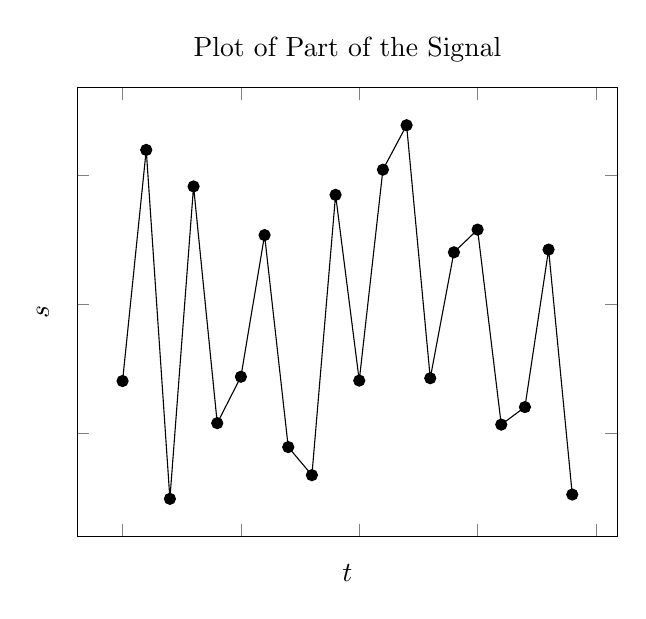
\begin{tikzpicture}

\begin{axis}[
    xlabel=\(t\),
    xticklabels={,,},
    ylabel=\(s\),
    yticklabels={,,},
    title={Plot of Part of the Signal},
]
    \addplot[
        color=black,
        mark=*,
    ] coordinates {
        (0, -0.59228515625)
        (1, 1.2001953125)
        (2, -1.505859375)
        (3, 0.9169921875)
        (4, -0.9189453125)
        (5, -0.55908203125)
        (6, 0.53955078125)
        (7, -1.1044921875)
        (8, -1.322265625)
        (9, 0.8515625)
        (10, -0.5888671875)
        (11, 1.046875)
        (12, 1.3916015625)
        (13, -0.5703125)
        (14, 0.406005859375)
        (15, 0.58203125)
        (16, -0.93017578125)
        (17, -0.79443359375)
        (18, 0.42724609375)
        (19, -1.47265625)
    };
\end{axis}

\end{tikzpicture}
\end{document}
